%%%%%%%%%%%%%%%%%%%%%%%%%%%%%%%%%%%%%%%%%%
%%%%%%%%%%%%%                 %%%%%%%%%%%%
%%%%%%%%%%%%%    EXERCISE 1   %%%%%%%%%%%%
%%%%%%%%%%%%%                 %%%%%%%%%%%%
%%%%%%%%%%%%%%%%%%%%%%%%%%%%%%%%%%%%%%%%%%
\begin{exercise}[Search]{For each of the following graph search strategies, work out the order in which states are expanded, as well as the path returned by graph search. In all cases, assume ties resolve in such a way that states with earlier alphabetical order are expanded first. Remember that in graph search, a state is expanded only once.
  \begin{enumerate}
    \item Depth-first search.
    \item Breadth-first search.
    \item Uniform cost search.
  \end{enumerate}
  \begin{figure}
    \begin{center}
    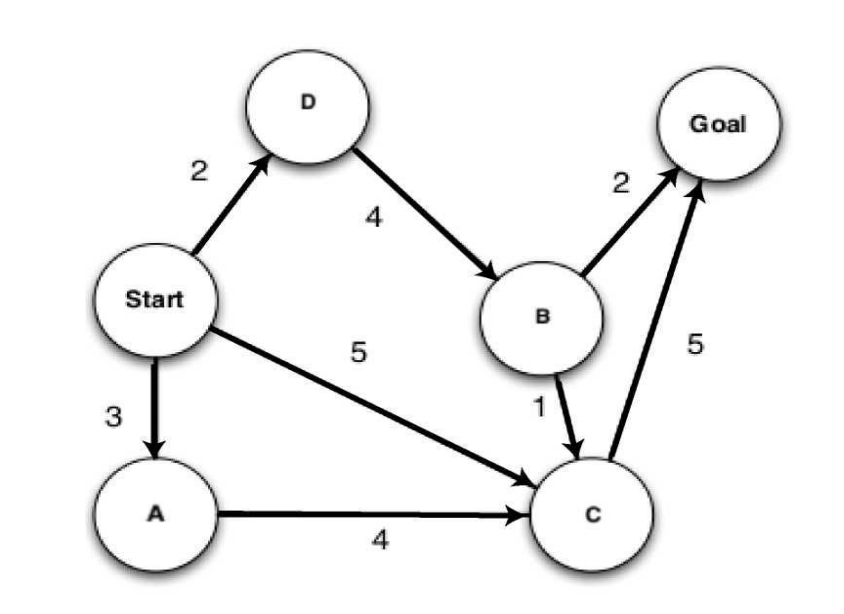
\includegraphics[width=8cm]{img/ex1.png}
    \end{center}
  \end{figure}
}
  \begin{solution}
  \par{~}
  \begin{enumerate}
    \item {
      Depth-First Search:

      Expand Order: Start $\rightarrow$ A $\rightarrow$ C $\rightarrow$ Goal

      Returned Path: Start $\rightarrow$ A $\rightarrow$ C $\rightarrow$ Goal
    }
    \item {
      Breadth-First Search:

      Expand Order: Start $\rightarrow$ A $\rightarrow$ C $\rightarrow$ D $\rightarrow$ Goal

      Returned Path: Start $\rightarrow$  C $\rightarrow$ Goal
    }
    \item {
      Uniform cost Search:

      Expand Order: Start $\rightarrow$ A $\rightarrow$ C $\rightarrow$ D $\rightarrow$ B $\rightarrow$ Goal

      Returned Path: Start $\rightarrow$ C $\rightarrow$ Goal
    }
  \end{enumerate}
  \end{solution}
  \label{ex1}
\end{exercise}


%%%%%%%%%%%%%%%%%%%%%%%%%%%%%%%%%%%%%%%%%%
%%%%%%%%%%%%%                 %%%%%%%%%%%%
%%%%%%%%%%%%%    EXERCISE 2   %%%%%%%%%%%%
%%%%%%%%%%%%%                 %%%%%%%%%%%%
%%%%%%%%%%%%%%%%%%%%%%%%%%%%%%%%%%%%%%%%%%
\begin{exercise}[Search]{2 SEARCH Which of the following are true and which are false?
  \begin{enumerate}
    \item Depth-first search always expands at least as many nodes as $A^{*}$ search with an admissible heuristic.
    \item $\mathrm{h}(\mathrm{n})=0$ is an admissible heuristic for the 8 -puzzle.
    \item $\mathrm{A}^{*}$ is of no use in robotics because percepts, states, and actions are continuous.
    \item Breadth-first search is complete even if zero step costs are allowed.
    \item Assume that a rook can move on a chessboard any number of squares in a straight line, vertically or horizontally, but cannot jump over other pieces. Manhattan distance is an admissible heuristic for the problem of moving the rook from square A to square $\mathrm{B}$ in the smallest number of moves.
  \end{enumerate}}
  \begin{solution}
  \par{~}
  \begin{enumerate}
    \item No, DFS may find the goal on initial exploration.
    \item Yes, since $0 \le h^{*}(n)$ anyway.
    \item No, delicate heuristic can be designed.
    \item Yes, BFS doesn't count costs.
    \item No, since $h^{*}(n)=2$ if there exists no obstacles, but the heuristic can be greater than 2 if the goal is far enough.
  \end{enumerate}
  \end{solution}
  \label{ex2}
\end{exercise}


%%%%%%%%%%%%%%%%%%%%%%%%%%%%%%%%%%%%%%%%%%
%%%%%%%%%%%%%                 %%%%%%%%%%%%
%%%%%%%%%%%%%    EXERCISE 3   %%%%%%%%%%%%
%%%%%%%%%%%%%                 %%%%%%%%%%%%
%%%%%%%%%%%%%%%%%%%%%%%%%%%%%%%%%%%%%%%%%%
\begin{exercise}[Search]{n vehicles occupy squares (1,1) through $(\mathrm{n}, 1)$ (i.e., the bottom row) of an $\mathrm{n}$ $\times \mathrm{n}$ grid. The vehicles must be moved to the top row but in reverse order; so the vehicle i that starts in $(\mathrm{i}, 1)$ must end up in $(\mathrm{n}-\mathrm{i}+1, \mathrm{n}) .$ On each time step, every one of the n vehicles can move one square up, down,left,or right,or stay put; but if a vehicle stays put, one other adjacent vehicle(but not more than one)can hop over it. Two vehicles cannot occupy the same square.
  \begin{enumerate}
    \item Calculate the size of the state space as a function of $n .$
    \item Calculate the branching factor as a function of $n .$
    \item Suppose that vehicle $i$ is at $\left(x_{i}, y\right) ;$ write a nontrivial admissible heuristic ha for the number of moves it will equire to get to its goal location $(n-i+1, n)$, assuming no other vehicles are on the grid.
    \item {Which of the following heuristics are admissible for the problem of moving all n vehicles to their destinations?Explain.
    \begin{itemize}
      \item $\sum_{i=1}^{n} h_{i}$
      \item $\max \left\{h_{1}, \ldots, h_{n}\right\}$
      \item $\min \left\{h_{1}, \ldots, h_{n}\right\}$
    \end{itemize}}
  \end{enumerate}}
  \begin{solution}
  \par{~}
  \begin{enumerate}
    \item {
      $n$ items can be distributed on $n\times n$ blanks. Hence there are $P_{n^2}^{n}$ states.
    }
    \item {
      For every vehicle, there are five choices to make, so for every state, there will be $5^n$ possible next-state. The branching factor is $5^n$
    }
    \item {
      A heuristic for single vehicle can be the Manhattan distance
      \begin{equation}
        h_i = \left| n - i + 1 - x_i\right| + \left| n - y_i \right|
      \end{equation}
    }
    \item {
      $\sum_{i=1}^{n} h_{i}$ cannot be an admissible heuristic since the vehicles can move simultaneously. As a result, it is likely that $h(n)>h^{*}(n)$

      $\max \left\{h_{1}, \ldots, h_{n}\right\}$ is an admissible heuristic, since if we want to make all the vehicles to their destinations, it must take at least the time for moving one particular vehicle to its destination. i.e. $h_{i}(n) \le h^{*}_{all}(n)$ for any i. Therefore, $\max \left\{h_{1}, \ldots, h_{n}\right\} \le h^{*}$.

      $\min \left\{h_{1}, \ldots, h_{n}\right\}$ is also admissible because $\min \left\{h_{1}, \ldots, h_{n}\right\} \le \max \left\{h_{1}, \ldots, h_{n}\right\} \le h^{*}$
    }
  \end{enumerate}
  \end{solution}
  \label{ex3}
\end{exercise}

%%%%%%%%%%%%%%%%%%%%%%%%%%%%%%%%%%%%%%%%%%
%%%%%%%%%%%%%                 %%%%%%%%%%%%
%%%%%%%%%%%%%    EXERCISE 4   %%%%%%%%%%%%
%%%%%%%%%%%%%                 %%%%%%%%%%%%
%%%%%%%%%%%%%%%%%%%%%%%%%%%%%%%%%%%%%%%%%%
\begin{exercise}[Search]{Develop a formal proof of correctness for alpha-beta pruning. To do this,
  consider the situation shown in Figure $5.18 .$ The question is whether to prune node $n_{j}$ which is a max-node and a descendant of node $n_{1}$ The basic idea is to prune it if and
  only if the minimax value of $n_{1}$ can be shown to be independent of the value of $n j .(35)$
  \begin{enumerate}
    \item Mode $n_{1}$ takes on the minimum value among its children: $n_{1}=\min \left(n_{2}, n_{21}, \ldots, n_{2 b_{2}}\right)$ Find a similar expression for $n_{2}$ and hence an expression for $n_{1}$ in terms of $n_{j}$.
    \item Let $l_{i}$ be the minimum (or maximum) value of the nodes to the $l e f t$ of node $n_{i}$ at depth $i$ whose minimax value is already known. Similarly, let $r_{i}$ be the minimum (or maximum) value of the unexplored nodes to the right of $n_{i}$ at depth $i .$ Rewrite your expression for $n_{1}$ in terms of the $l_{i}$ and $r_{i}$ values.
    \item Now reformulate the expression to show that in order to affect $n_{1}, n_{j}$ must not exceed a certain bound derived from the $l_{i}$ values.
    \item Repeat the process for the case where $n_{j}$ is a min-node.
  \end{enumerate}
  \begin{figure}
    \begin{center}
      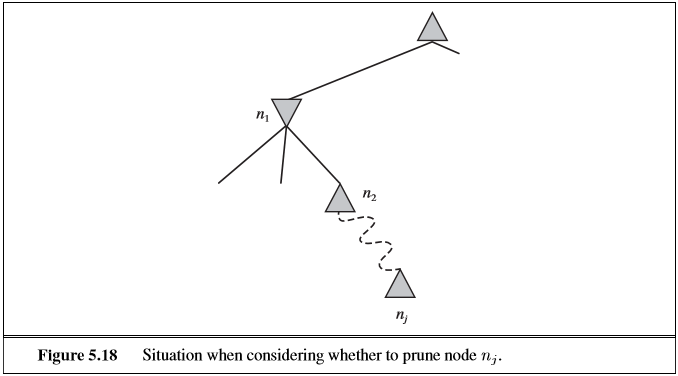
\includegraphics[width=12cm]{img/ex1-1.png}
    \end{center}
  \end{figure}
  }
  \begin{solution}
  \par{~}
  \begin{enumerate}
    \item {

    }
    \item {
      
    }
    \item {
      
    }
    \item {
      
    }
  \end{enumerate}
  \end{solution}
  \label{ex4}
\end{exercise}